The driver will need to be able to directly control several electronic systems while in a driving position. These systems include the Electric Vehicles directional indicators, the speed of the vehicle, the direction the vehicle is travelling in as well as being able to place the car in its safe state. While in its safe state the batteries must be isolated from the rest of the vehicle. The driver will also have to be able to exit the safe state while in the drivers seat. 

Apart from being able to control systems the driver must also be relayed important information such as the speed of the vehicle, the state of charge of the batteries as well as being alerted of any faults which develop.

\subsection{Directional Indicators}

To comply with regulations the vehicle must have indicators which alert other road users of the drivers intentions. [REWORD A BIT CLUNKY] The indicators must pulse on and off at 90 pulses per minute when the indicators are active. 

\begin{figure}[H]
%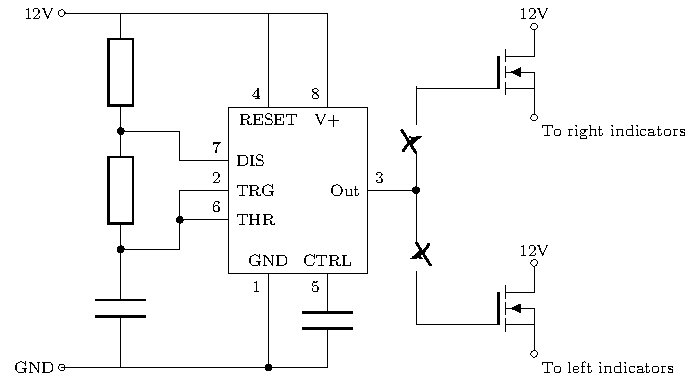
\includegraphics[width=\columnwidth]{figures/555Circuit}% Image
\begin{center}
%\documentclass{standalone}
%\usepackage[latin1]{inputenc}
%\usepackage{amsmath}
%\usepackage{amsfonts}
%\usepackage{amssymb}
%\usepackage{makeidx}
%\usepackage{graphicx}
%\usepackage{caption}
%\usepackage{subcaption}
%\usepackage{float}
%\usepackage{wrapfig}
%\usepackage[left=1.00in, right=1.00in, top=1.00in, bottom=1.00in]{geometry}
%\usepackage{tikz}
%\usepackage{circuitikz}
%\usepackage{newclude}
%\usepackage{calc}
%\usetikzlibrary{matrix,positioning,calc,intersections,arrows,fadings}

%\begin{document}
		
  	\tikzstyle{icdev}=[draw, text width=6em, minimum height=8em]
  	
    \begin{tikzpicture}[every node/.style = {font = \footnotesize},european]
    \draw (0,6) node[left]{12V}  % from top Vcc to bottom Gnd
    to[short,o-,] (1,6)
    to[R] (1,4) 
    to[R] (1,2)
    to[C] (1,0)
    to[short,-o] (0,0) node[left]{GND}
    ;
    \draw (4,3) node[icdev] (555)  {};  % position IC device body
    % top terminal lines/pins - 4 RESET, 8 V+
    \path [draw](1,6) -| ($(555.north)+(-0.5,0)$) node[below]{RESET} node[above left]{4};
    \path [draw](1,6) -| ($(555.north)+(0.5,0)$) node[below]{V+} node[above left] {8};
    % leftside terminal lines/pins - 7 DIS, 6 THR, 2 TRG
    \path [draw](2,4) |- ($(555.west)+(0,2/4)$) node[right]{DIS} node[above left]{7};
    \path [draw](2,2) |- ($(555.west)+(0,0/4)$) node[right]{TRG} node[above left]{2};
    \path [draw](2,2) |- ($(555.west)+(0,-2/4)$) node[right]{THR} node[above left]{6};
    \draw (1,4) 
    to[short,*-] (2,4);
    \draw (1,2) 
    to[short,*-] (2,2)
    to[short,-*] (2,2.5);
    
    % bottom terminal lines/pins - 1 GND, 5 CTRL
    \path [draw](0,0) -| ($(555.south)+(-0.5,0)$) node[above]{GND} node[below left]{1};
    \draw(0,0) to[short,-*] (3.5,0)
    to[short] (4.5,0)
    to[C]($(555.south)+(0.5,0)$)  
    node[above]{CTRL} node[below left]{5}; % C = 10nf

    % rightside terminal line/pin - 3 out
    \draw (555.east) node[left]{Out} node[above right]{3}
    to[short,-*] (6,3);
    
    %Position Transistors
    \draw (8,1) node[nigfete] (leftfet) {};
    \draw (8,5) node[nigfete] (rightfet) {};
    
    %Switches and transistors
    \draw (6,3) 
    to[closing switch] (6,0.75) 
    |- (leftfet.G);
    \draw (6,3)
    to[closing switch] (6,4.75)
    |- (rightfet.G);
    
    %Connections on transistors
    \draw (leftfet.S) node[below right]{To left indicators}
    to[short,-o] (leftfet.S);
    \draw (rightfet.S) node[below right]{To right indicators}
    to[short,-o] (rightfet.S);
    \draw (leftfet.D) node[above]{12V}
    to[short,-o] (leftfet.D);
    \draw (rightfet.D) node[above]{12V}
    to[short,-o] (rightfet.D);
    \end{tikzpicture}
%\end{document}

\caption{Wiring Diagram of the Indicator Drivers}
\label{Fig:IndicatorWiring}
\end{center}
\end{figure}

As shown in Figure \ref{Fig:IndicatorWiring} a 555 timer is used to control a 12V bus which powers the LEDs. Due to the curvature on the front of the vehicle the front indicators are flexible LED strips which we can mould to the vehicles shape. However, the rear indicators use a specially designed LED strip with a constant current driver. [NOT SURE WHETHER TO GO INTO MORE DETAIL OF THE CONST. CURRENT]

\subsection{Brake Lights}

Rear brake lights must be fitted to the vehicle which activate automatically when the driver activates the brakes. In order to detect when the driver applies the brakes a micro switch is fitted to the brake pedal and hand brake lever. The switches are wired in parallel and control the power going to the brake light drivers. 

\begin{figure}[H]
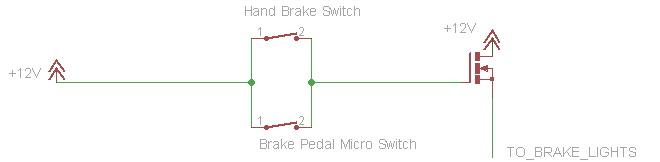
\includegraphics[width=\columnwidth]{figures/BrakeLightControl}%
\caption{Brake Light Control Schematic}
\label{Fig:BrakeLightsWiring}
\end{figure}

\subsection{Controlling the Motor}
In order to set the speed of the vehicle the motor controller needs to be sent messages with a target speed for the motor. The motor controller uses this information to control the amount of power fed into the motor in order to control its speed. The messages are sent via the CAN bus of the vehicle allowing for any device attached to the CAN bus to have access to information such as speed and motor power consumption. 

As the driver would likely be travelling at roughly the same speed for the entirety of their three hour sessions it was decided that a cruise control system would be most suitable. Where the driver holds down a dead man switch and controls the speed using a potentiometer located near the driver.

The device which takes take of all the driver inputs is known as the main controller. The main controller reads the state of the accelerator pedal which acts as a dead man switch. If the accelerator is pressed the main controller then reads the value of the speed control which acts as an analogue input to the main controller. After encoding the analogue value it is sent over the CAN bus to the motor controller. A third input is attached to the main controller which controls whether the motor will go forwards, backwards or act as a brake. This tristate switch when in the forward state will cause the main controller to behave as previously described. When in the brake state it will cause the main controller to only send the motor controller a command which tells it to keep the motor stationary. This command will be sent until the switch is placed into another state. Finally, if the switch is placed into the reverse position the main controller will activate the rear view camera as well as altering the speed command that is sent to the motor controller such that it will cause the motor to rotate backwards.

\begin{figure}[H]
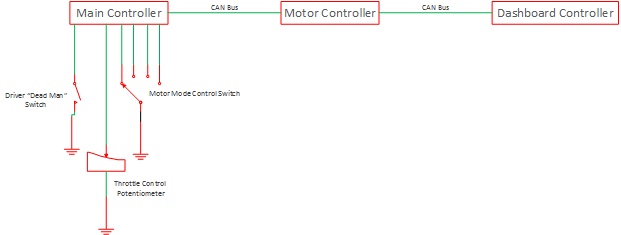
\includegraphics[width=\columnwidth]{figures/MotorControlDiagram.png}%
\caption{Motor Communication Diagram}
\label{Fig:MotorControl}
\end{figure}

\subsection{Vehicle Safe State}
The electric vehicles safe state causes the only conductors that leave the battery box to be galvanically isolated from the batteries. It also causes the solar array to be disconnected from the electrical systems. 

In order to enter this state a normally closed button wired in series to the relay control mechanism is pressed. This will interrupt power to the relay control which will cause the relays to return to their normally open position.

\begin{figure}[H]
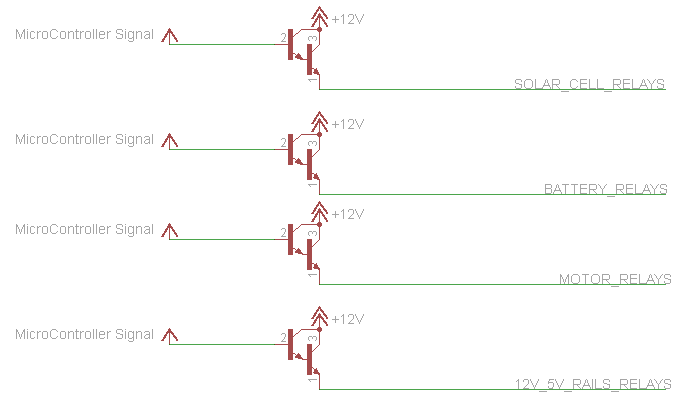
\includegraphics[width=\columnwidth]{figures/RelayControl.png}%
\caption{Relay Control Mechanism}
\label{Fig:RelayControl}
\end{figure}

In order to close a relay a 5V signal must be sent from a micro controller which feeds into a Darlington Transistor which controls a 12V signal which is then wired up to the coils of normally open relays. So when both a 5V signal and a 12V rail is attached the relays will close. TO enter the safe state the 12V or the 5V rail must be deactivated which is done by controlling a relay wired in series to the rails.

Only a few devices can control the 5V signal which can be used to disconnect individual relays. These devices are the main controller and a second controller which operates many of the safety systems. The second controller is interfaced with temperature sensors attached to each cell on the batteries through a one wire bus so it is able to isolate parts of the vehicle automatically if for instance a battery gets too hot it can place the vehicle to the safe state. Or if a part of the array is malfunctioning it can isolate that part of the array as well as alerting the driver to the malfunction.

Once in the safe state the problem of exiting the safe state arises. Both the 12V and 5V rail have to be enabled to exit the safe state, as opposed to entering which only required disabling one of the rails. Furthermore, the driver must be able to do this from within the drivers seat meaning the system must be galvanically isolated. In order to do this a seperate isolated DCDC converter is used. This supply can control the relays necessary to exit the safe state and so by wiring up a mechanical switch the driver can easily exit the safe state

\begin{figure}[H]
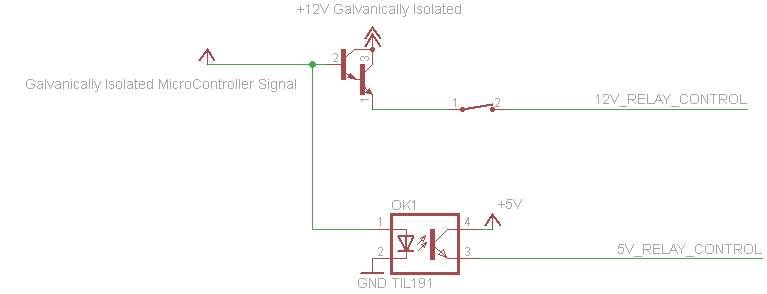
\includegraphics[width=\columnwidth]{figures/SafeStateIsolated.png}%
\caption{Galvanically Isolated Relay Control}
\label{Fig:IsolatedControl}
\end{figure}
